\documentclass[english]{SPFShortReport}
\usepackage{subfigure}
\usepackage{spfFigures}
\usepackage{longtable}
\usepackage{url}
\usepackage{gensymb}
\usepackage[yyyymmdd,hhmmss]{datetime}
\reportName{Python calculation for heat pump SIN-130TE}
\reportSubName{Parametric Heat Pump calculation} 
\reportDate{\today \hspace{0.1cm} at: \currenttime \hspace{0.1cm} h} 
\author{Dani Carbonell}
\address{dani.carbonell@solarenergy.ch}
\begin{document}
\begin{table}[!ht]
\begin{small}
\caption{Fitted coefficients for the heat pump.}
\begin{center}
\resizebox{12cm}{!} 
{
\begin{tabular}{l | c c } 
\hline
\hline
Coefficient &Description & \\ 
 & &$[kW]$\\ 
\hline
$PQ_{1}$ & \emph{$1^{st}$ condenser polynomial coefficient}  & 1.1017e+02    \\ 
$PQ_{2}$ & \emph{$2^{st}$ condenser polynomial coefficient}  & 8.3243e+02    \\ 
$PQ_{3}$ & \emph{$3^{st}$ condenser polynomial coefficient}  & 4.1398e+02    \\ 
$PQ_{4}$ & \emph{$4^{st}$ condenser polynomial coefficient}  & -2.2461e+00    \\ 
$PQ_{5}$ & \emph{$5^{st}$ condenser polynomial coefficient}  & 3.3288e+02    \\ 
$PQ_{6}$ & \emph{$6^{st}$ condenser polynomial coefficient}  & -2.1955e+03    \\ 
\hline
$PCOP_{1}$ & \emph{$1^{st}$ COP polynomial coefficient}  & 5.2782e+00    \\ 
$PCOP_{2}$ & \emph{$2^{st}$ COP polynomial coefficient}  & 3.3528e+01    \\ 
$PCOP_{3}$ & \emph{$3^{st}$ COP polynomial coefficient}  & 2.0320e+00    \\ 
$PCOP_{4}$ & \emph{$4^{st}$ COP polynomial coefficient}  & -7.8493e+01    \\ 
$PCOP_{5}$ & \emph{$5^{st}$ COP polynomial coefficient}  & 7.6224e+00    \\ 
$PCOP_{6}$ & \emph{$6^{st}$ COP polynomial coefficient}  & -8.5718e+01    \\ 
\hline
$\dot m_{cond}$ & 21000.00 $[kg/h]$\\ 
$\dot m_{evap}$ & 21000.00 $[kg/h]$\\ 
\hline
$COP_{nom}$ (B0W35)& 4.12 \\ 
$Q_{c,nom}$ (B0W35)& 122.04 kW\\ 
$COP_{nom}$ (B2W35)& 4.30 \\ 
$Q_{c,nom}$ (B2W35)& 127.77 kW\\ 
$COP_{nom}$ (B10W35)& 5.00 \\ 
$Q_{c,nom}$ (B10W35)& 151.00 kW\\ 
\hline
\hline
\end{tabular}
}
\label{CoefTable}
\end{center}
\end{small}
\end{table}
\begin{table}[!ht]
\begin{small}
\caption{Predicting results of the heat pump.}
\begin{center}
\resizebox{12cm}{!} 
{
\begin{tabular}{l | c c c c c c c c c c c } 
\hline
\hline
$T_{evap,in}$ &$T_{evap,out}$ &$T_{cond,in}$ &$T_{cond,out}$ &$COP$ &$Q_{cond}$ &$Q_{evap}$ &$W_{comp}$ &$\dot m_{cond}$ &$\dot m_{evap}$ &$\Delta T_{evap}$ &$\Delta T_{cond}$ \\ 
$^oC$ &$^oC$ &$^oC$ &$^oC$ &$[-]$ &$[kW]$ &$[kW]$ &$[kW]$ &kg/h &kg/h &K &K\\ 
\hline
-7.00 & -10.42 & 25.77 & 30.00 & 3.79 & 103.36 & 76.06 & 27.30 & 21000 & 21000 & 3.4 & 4.2\\ 
-7.00 & -10.14 & 34.64 & 38.75 & 3.29 & 100.38 & 69.88 & 30.51 & 21000 & 21000 & 3.1 & 4.1\\ 
-7.00 & -9.58 & 43.69 & 47.50 & 2.62 & 93.15 & 57.54 & 35.61 & 21000 & 21000 & 2.6 & 3.8\\ 
-7.00 & -8.59 & 52.90 & 56.25 & 1.76 & 81.77 & 35.29 & 46.48 & 21000 & 21000 & 1.6 & 3.3\\ 
-7.00 & -5.96 & 62.22 & 65.00 & 0.75 & 67.97 & -23.20 & 91.17 & 21000 & 21000 & -1.0 & 2.8\\ 
-4.00 & -7.78 & 25.43 & 30.00 & 4.05 & 111.78 & 84.21 & 27.57 & 21000 & 21000 & 3.8 & 4.6\\ 
-4.00 & -7.51 & 34.29 & 38.75 & 3.54 & 108.89 & 78.09 & 30.80 & 21000 & 21000 & 3.5 & 4.5\\ 
-4.00 & -6.96 & 43.34 & 47.50 & 2.84 & 101.74 & 65.90 & 35.85 & 21000 & 21000 & 3.0 & 4.2\\ 
-4.00 & -5.99 & 52.55 & 56.25 & 1.96 & 90.44 & 44.26 & 46.18 & 21000 & 21000 & 2.0 & 3.7\\ 
-4.00 & -3.67 & 61.88 & 65.00 & 0.91 & 76.27 & -7.26 & 83.53 & 21000 & 21000 & -0.3 & 3.1\\ 
-1.00 & -5.15 & 25.08 & 30.00 & 4.32 & 120.26 & 92.45 & 27.81 & 21000 & 21000 & 4.2 & 4.9\\ 
-1.00 & -4.88 & 33.94 & 38.75 & 3.78 & 117.46 & 86.41 & 31.05 & 21000 & 21000 & 3.9 & 4.8\\ 
-1.00 & -4.34 & 42.98 & 47.50 & 3.06 & 110.41 & 74.36 & 36.04 & 21000 & 21000 & 3.3 & 4.5\\ 
-1.00 & -3.39 & 52.19 & 56.25 & 2.16 & 99.17 & 53.26 & 45.91 & 21000 & 21000 & 2.4 & 4.1\\ 
-1.00 & -1.30 & 61.53 & 65.00 & 1.09 & 84.78 & 6.71 & 78.07 & 21000 & 21000 & 0.3 & 3.5\\ 
2.00 & -2.53 & 24.73 & 30.00 & 4.60 & 128.80 & 100.78 & 28.02 & 21000 & 21000 & 4.5 & 5.3\\ 
2.00 & -2.26 & 33.59 & 38.75 & 4.03 & 126.09 & 94.83 & 31.26 & 21000 & 21000 & 4.3 & 5.2\\ 
2.00 & -1.73 & 42.63 & 47.50 & 3.29 & 119.13 & 82.93 & 36.20 & 21000 & 21000 & 3.7 & 4.9\\ 
2.00 & -0.80 & 51.83 & 56.25 & 2.36 & 107.97 & 62.31 & 45.66 & 21000 & 21000 & 2.8 & 4.4\\ 
2.00 & 1.13 & 61.18 & 65.00 & 1.26 & 93.44 & 19.47 & 73.97 & 21000 & 21000 & 0.9 & 3.8\\ 
5.00 & 0.09 & 24.38 & 30.00 & 4.87 & 137.41 & 109.21 & 28.21 & 21000 & 21000 & 4.9 & 5.6\\ 
5.00 & 0.36 & 33.24 & 38.75 & 4.29 & 134.79 & 103.34 & 31.45 & 21000 & 21000 & 4.6 & 5.5\\ 
5.00 & 0.89 & 42.27 & 47.50 & 3.52 & 127.92 & 91.59 & 36.33 & 21000 & 21000 & 4.1 & 5.2\\ 
5.00 & 1.79 & 51.47 & 56.25 & 2.57 & 116.83 & 71.40 & 45.43 & 21000 & 21000 & 3.2 & 4.8\\ 
5.00 & 3.59 & 60.82 & 65.00 & 1.44 & 102.22 & 31.44 & 70.77 & 21000 & 21000 & 1.4 & 4.2\\ 
8.00 & 2.71 & 24.02 & 30.00 & 5.15 & 146.08 & 117.71 & 28.37 & 21000 & 21000 & 5.3 & 6.0\\ 
8.00 & 2.97 & 32.88 & 38.75 & 4.54 & 143.55 & 111.94 & 31.61 & 21000 & 21000 & 5.0 & 5.9\\ 
8.00 & 3.49 & 41.90 & 47.50 & 3.75 & 136.77 & 100.33 & 36.44 & 21000 & 21000 & 4.5 & 5.6\\ 
8.00 & 4.38 & 51.10 & 56.25 & 2.78 & 125.77 & 80.55 & 45.21 & 21000 & 21000 & 3.6 & 5.1\\ 
8.00 & 6.07 & 60.45 & 65.00 & 1.63 & 111.11 & 42.90 & 68.21 & 21000 & 21000 & 1.9 & 4.5\\ 
11.00 & 5.33 & 23.67 & 30.00 & 5.43 & 154.82 & 126.30 & 28.52 & 21000 & 21000 & 5.7 & 6.3\\ 
11.00 & 5.58 & 32.52 & 38.75 & 4.80 & 152.38 & 120.62 & 31.76 & 21000 & 21000 & 5.4 & 6.2\\ 
11.00 & 6.10 & 41.54 & 47.50 & 3.99 & 145.69 & 109.16 & 36.52 & 21000 & 21000 & 4.9 & 6.0\\ 
11.00 & 6.97 & 50.74 & 56.25 & 2.99 & 134.76 & 89.75 & 45.01 & 21000 & 21000 & 4.0 & 5.5\\ 
11.00 & 8.57 & 60.09 & 65.00 & 1.82 & 120.09 & 53.99 & 66.11 & 21000 & 21000 & 2.4 & 4.9\\ 
14.00 & 7.94 & 23.31 & 30.00 & 5.71 & 163.61 & 134.97 & 28.65 & 21000 & 21000 & 6.1 & 6.7\\ 
14.00 & 8.19 & 32.15 & 38.75 & 5.06 & 161.26 & 129.38 & 31.88 & 21000 & 21000 & 5.8 & 6.6\\ 
14.00 & 8.70 & 41.17 & 47.50 & 4.23 & 154.66 & 118.07 & 36.59 & 21000 & 21000 & 5.3 & 6.3\\ 
14.00 & 9.55 & 50.37 & 56.25 & 3.21 & 143.83 & 99.01 & 44.82 & 21000 & 21000 & 4.4 & 5.9\\ 
14.00 & 11.09 & 59.72 & 65.00 & 2.01 & 129.16 & 64.83 & 64.34 & 21000 & 21000 & 2.9 & 5.3\\ 
17.00 & 10.54 & 22.94 & 30.00 & 6.00 & 172.47 & 143.71 & 28.76 & 21000 & 21000 & 6.5 & 7.1\\ 
17.00 & 10.79 & 31.79 & 38.75 & 5.32 & 170.21 & 138.23 & 31.99 & 21000 & 21000 & 6.2 & 7.0\\ 
17.00 & 11.29 & 40.80 & 47.50 & 4.47 & 163.71 & 127.06 & 36.65 & 21000 & 21000 & 5.7 & 6.7\\ 
17.00 & 12.13 & 49.99 & 56.25 & 3.43 & 152.96 & 108.33 & 44.63 & 21000 & 21000 & 4.9 & 6.3\\ 
17.00 & 13.61 & 59.34 & 65.00 & 2.20 & 138.32 & 75.49 & 62.82 & 21000 & 21000 & 3.4 & 5.7\\ 
20.00 & 13.15 & 22.58 & 30.00 & 6.28 & 181.40 & 152.53 & 28.87 & 21000 & 21000 & 6.9 & 7.4\\ 
20.00 & 13.39 & 31.42 & 38.75 & 5.59 & 179.23 & 147.14 & 32.08 & 21000 & 21000 & 6.6 & 7.3\\ 
20.00 & 13.88 & 40.43 & 47.50 & 4.71 & 172.82 & 136.12 & 36.69 & 21000 & 21000 & 6.1 & 7.1\\ 
20.00 & 14.71 & 49.62 & 56.25 & 3.65 & 162.16 & 117.70 & 44.45 & 21000 & 21000 & 5.3 & 6.6\\ 
20.00 & 16.14 & 58.96 & 65.00 & 2.40 & 147.55 & 86.03 & 61.51 & 21000 & 21000 & 3.9 & 6.0\\ 
\hline
\hline
\end{tabular}
}
\label{ResultsTable}
\end{center}
\end{small}
\end{table}
\begin{figure}[!ht]
\begin{center}
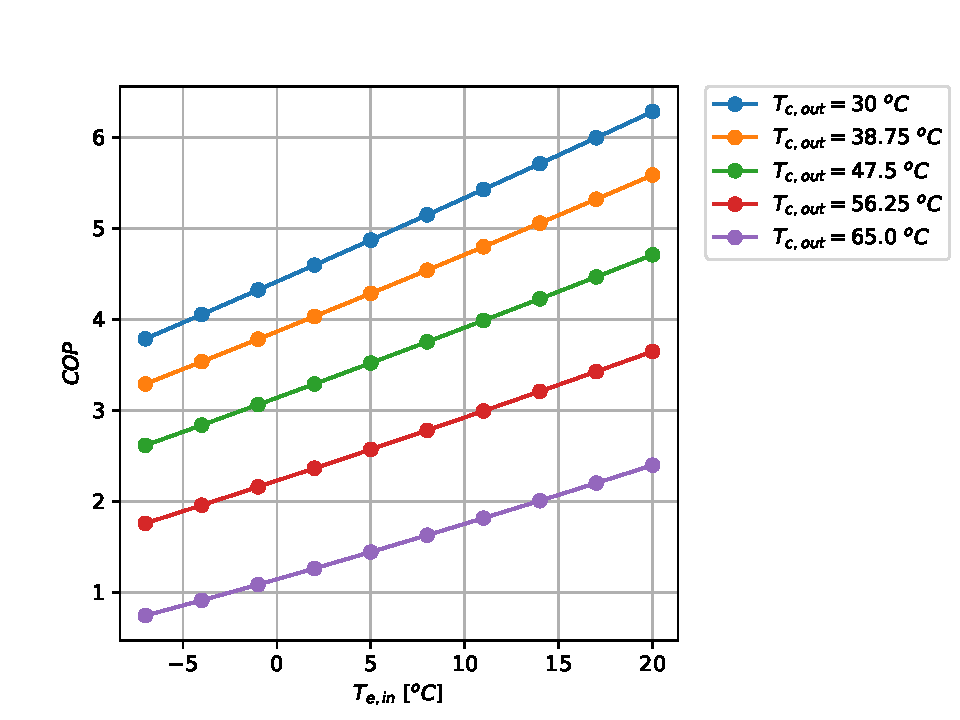
\includegraphics[width=1\textwidth]{C:/Daten/spfPackages/GIT/spfTrnsysFiles/HeatPump/BrineToWater/Walter Meier/SIN-130TE/SIN-130TE-Cop.pdf}
\caption{COP Results for the heat pump at the selected points}
\label{COPFig}
\end{center}
\end{figure}
\begin{figure}[!ht]
\begin{center}
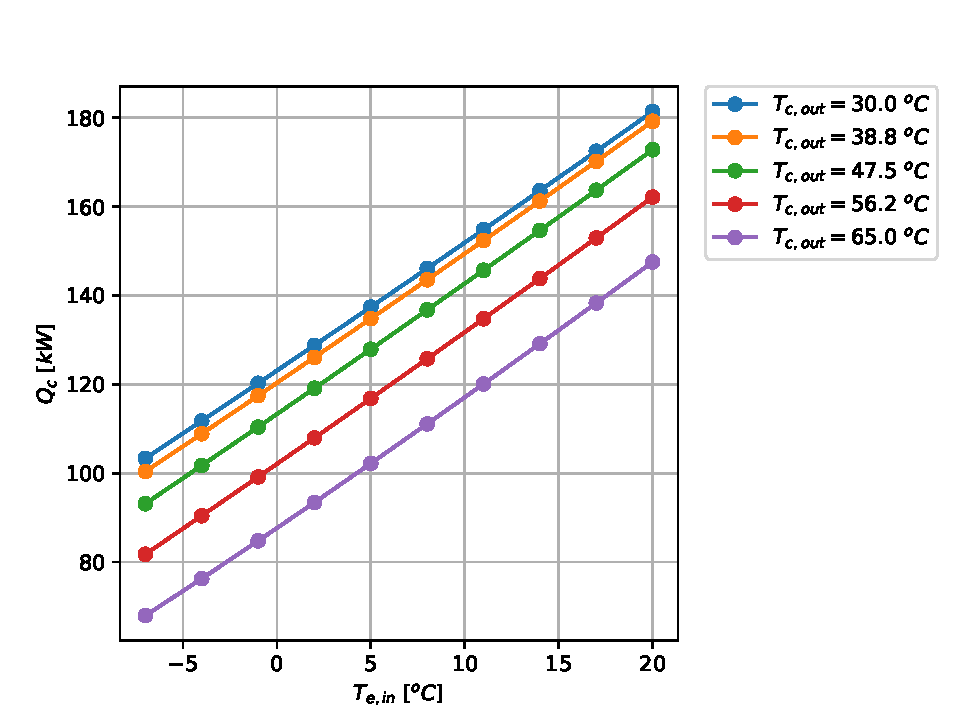
\includegraphics[width=1\textwidth]{C:/Daten/spfPackages/GIT/spfTrnsysFiles/HeatPump/BrineToWater/Walter Meier/SIN-130TE/SIN-130TE-Qc.pdf}
\caption{$Q_c$ Results for the heat pump at the selected points}
\label{QcFig}
\end{center}
\end{figure}
\end{document}
